\documentclass[12pt, a4paper]{article}
\usepackage{graphicx}
\usepackage{amsmath}
\usepackage{hyperref}
\usepackage{geometry}
\geometry{margin=1in}
\usepackage{setspace}
\usepackage{booktabs}
\usepackage{caption}
\usepackage{float}
\setstretch{1.2}

\title{\textbf{Deep Learning-Based Leaf Diseases Detection in Indoor Ornamental Plants: A Full-Stack AI Platform}}
\author{Nishad Mahmud \and Ruma}
\date{}

\begin{document}

\maketitle

\begin{abstract}
Accurate leaf disease detection in indoor ornamental plants remains a critical challenge due to reliance on subjective visual inspection and the high cost of molecular diagnostics. This project addresses the need for an efficient and lightweight system to monitor plant health and prevent disease spread in controlled environments. The main objective is to develop and evaluate a comprehensive end-to-end detection model, based on modern YOLO architectures, to identify and localize nine disease and healthy classes across three species: Money Plant, Snake Plant, and Spider Plant. A custom dataset of 787 high-resolution images was collected, annotated, and expanded to 3,935 images via systematic augmentation. Three variants—YOLOv8s, YOLOv9s, and YOLOv11s—were trained. YOLOv11s achieved superior performance, recording 97.4\% mAP@50 and 89.3\% mAP@50-95. 

To bridge the gap between academic research and real-world utility, this project extends the YOLOv11s model into a production-ready, Progressive Web Application (PWA). Developed utilizing Next.js for the frontend and FastAPI for the backend inference engine, the platform enables real-time, hardware-benchmarked inference directly from mobile or desktop devices. To enhance interpretability and user trust, occlusion sensitivity and RISE (Randomized Input Sampling for Explanation) analyses were dynamically integrated into the user interface, confirming that the model focuses on disease-relevant leaf regions while suppressing background features. The resulting framework delivers an accurate, interpretable, and highly accessible solution for indoor plant disease monitoring.
\end{abstract}

\newpage
\tableofcontents
\newpage

\section{Introduction}
Plant diseases cause substantial losses in agricultural productivity, directly affecting food security and farmer livelihoods. Traditional detection methods, which rely on human expertise, are often subjective, error-prone, and inefficient when scaled to large farming systems or indoor ornamental care. Advances in computer vision and deep learning have made automated plant disease detection a promising approach, offering rapid, accurate, and scalable solutions for practical applications.

Although several deep learning models have been applied in this domain, challenges persist due to limited datasets, lack of standardized annotations, and insufficient interpretability of model predictions. Furthermore, many existing research papers focus strictly on single architectures or small-scale datasets, leaving the trained models isolated as academic exercises without practical deployment mechanisms. The "black-box" characteristics of deep neural networks also remain a source of concern regarding trust and transparency in agricultural applications.

Building on the progress of advanced object detection architectures, the present study leverages YOLOv8s, YOLOv9s, and YOLOv11s to address multi-class plant disease detection. To ensure the model is practically usable, we engineered a full-stack Progressive Web App (PWA) bridging the high-performance AI inference engine with an intuitive, mobile-friendly user interface. 

The primary objectives of this project are:
\begin{itemize}
    \item Development of an augmented and annotated dataset for plant disease detection with improved diversity and representativeness.
    \item Implementation and comparative evaluation of YOLOv8s, YOLOv9s, and YOLOv11s models on multi-class indoor plant disease detection.
    \item Engineering a modern, scalable web architecture (Next.js and FastAPI) to serve the model to end-users efficiently, complete with client-side image compression and offline PWA capabilities.
    \item Integration of interpretability methods (occlusion sensitivity and RISE analysis) directly into the UI to enhance transparency, trust, and real-world deployment potential.
\end{itemize}

\section{Literature Review}
Historically, plant disease detection relied on farmers' and experts' visual examination, a subjective and error-prone process. Molecular diagnostic methods such as FISH, ELISA, PCR, and LAMP improved sensitivity and reliability but remain costly and time-consuming. 

Recent research examines machine learning (ML) and deep learning (DL) techniques for the detection, categorization, and severity assessment of agricultural diseases. Conventional ML models such as SVM, KNN, Random Forest, and ANN have been employed, but DL methodologies—particularly CNNs and transfer learning architectures like AlexNet, VGG16, ResNet, and Inception—have consistently attained superior accuracy. Object detection frameworks like YOLO (v4-v8) and Faster R-CNN, combined with advanced backbones, enabled multi-class detection across numerous species, achieving mAP scores of 92-98\% on datasets such as PlantVillage.

Lightweight solutions balance accuracy and efficiency. Integrating color segmentation with CNNs has historically reached high accuracy in detecting food crop diseases while providing faster predictions. Beyond food crops, ornamental and indoor plants have gained attention. A YOLOv5-based system for money plant disease achieved 93\% accuracy, offering mobile-friendly deployment. Further improvements using attention mechanisms boosted performance significantly. In this work, we deploy a YOLOv11-based detector integrated into a full-stack software environment to provide a holistic, end-to-end solution.

\section{Methodology and Machine Learning Pipeline}
\subsection{Data Collection}
A custom dataset was created consisting of three species of indoor plants: Money Plant, Snake Plant, and Spider Plant. The dataset includes 787 high-resolution images across nine different categories: Money Plant Bacterial Wilt Disease, Money Plant Healthy, Money Plant Manganese Toxicity, Snake Plant Anthracnose, Snake Plant Healthy, Snake Plant Leaf Withering, Spider Plant Fungal Leaf Spot, Spider Plant Healthy, and Spider Plant Leaf Tip Necrosis. In each category, there are 81 to 93 images, ensuring data balance. Photographs were taken in various plant nurseries during normal daylight conditions, capturing real changes in light and background.

\subsection{Dataset Annotation and Preprocessing}
The dataset was prepared for object detection by manually annotating all images. Healthy leaves were marked with a single bounding box around the whole leaf and categorized appropriately. Diseased leaves were similarly annotated and labeled with the corresponding disease category, enabling the model to learn full-leaf disease classification. Images and annotations were exported in YOLO format and resized to $640 \times 640$ pixels with padding to preserve the aspect ratio.

\subsection{Data Augmentation}
To mitigate the small original dataset size and enhance generalization, a systematic augmentation pipeline was implemented using the Albumentations library. The dataset was expanded fivefold to a total of 3,935 images. Augmentations included horizontal and vertical flipping, 90-degree rotations, randomized zooming, and photometric transformations such as brightness and exposure variations. 

\subsection{YOLO Model Configurations}
Three state-of-the-art YOLO variants—YOLOv8, YOLOv9, and YOLOv11—were studied. As the main baseline, YOLOv11 brings together the C3k2 block backbone with hierarchical feature extraction, SPPF modules for multi-scale feature aggregation, and the C2PSA spatial attention module to enhance feature representation. All models were trained with a $640\times640$ input size and optimized using the AdamW optimizer over 100 epochs.

\section{System Architecture and Web Application}
The transition from an academic model to a production-ready system required a robust, dual-tier software architecture comprising a FastAPI backend and a Next.js frontend.

\subsection{Backend Inference Engine (FastAPI)}
The backend is architected using FastAPI, providing high-performance RESTful endpoints. The backend lifecycle includes:
\begin{itemize}
    \item \textbf{Model Initialization:} PyTorch-based YOLO weights are pre-loaded into memory during server startup to eliminate cold-start latency.
    \item \textbf{Inference Pipeline:} Uploaded images are dynamically resized and letterboxed to maintain aspect ratios before being passed through the neural network. 
    \item \textbf{Hardware Benchmarking:} The backend actively monitors RAM utilization, CPU/GPU latency, and preprocessing times, returning these metrics alongside the bounding box coordinates to provide users with system performance insights.
\end{itemize}

\subsection{Frontend Dashboard (Next.js)}
The user interface is built using Next.js 16 with the App Router and TailwindCSS for responsive design.
\begin{itemize}
    \item \textbf{Client-Side Image Compression:} High-resolution smartphone images (often exceeding 10MB) are compressed entirely within the browser using the \texttt{browser-image-compression} library. This ensures images are reduced to under 1MB before network transmission, drastically reducing payload times on weak mobile networks.
    \item \textbf{Mobile-First Camera Integration:} The UI provides native camera access via HTML5 \texttt{capture} attributes, allowing users to seamlessly snap photos of their plants directly from the web browser.
\end{itemize}

\subsection{Progressive Web Application (PWA)}
To simulate a native application experience, the web platform was converted into a Progressive Web App (PWA) using Serwist. 
\begin{itemize}
    \item \textbf{Service Worker Caching:} All static assets (JavaScript bundles, CSS, fonts, and layout shells) are heavily cached on the device.
    \item \textbf{Installability:} Users are prompted to ``Add to Home Screen,'' installing the platform as a standalone app with a customized app icon and hidden browser URL bars, creating an immersive, app-like experience.
\end{itemize}

\subsection{Interactive Explainable AI (XAI)}
The ``black-box'' nature of the YOLO architecture is mitigated by generating XAI heatmaps upon user request through the dashboard. The backend dynamically runs Occlusion Sensitivity and RISE (Randomized Input Sampling for Explanation) algorithms on the uploaded image and streams the resulting heatmaps back to the frontend. This visual proof enables the user to verify that the model is indeed looking at the disease lesions rather than background artifacts.

\section{Experiments and Results}

\subsection{Quantitative Results of All Models}
The detection performance was assessed on the test split of the augmented dataset. YOLOv11s achieved the highest mAP@50 (97.4\%), slightly outperforming YOLOv8s (97.1\%) and YOLOv9s (96.6\%). When evaluated across stricter thresholds (mAP@50–95), YOLOv11s again led with 89.3\%, indicating superior robustness under varying overlap conditions. For classification reliability, YOLOv11s reached the highest Precision (93.7\%) and Recall (96.7\%).

\begin{figure}[H]
\centerline{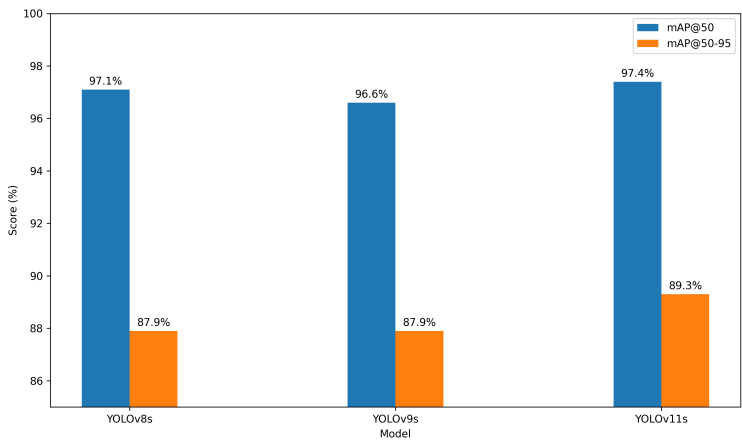
\includegraphics[width=0.7\textwidth]{images/944ce8e908c4deeeed7c76650af6adef-image.png}}
\caption{mAP@50 and mAP@50–95 comparison across YOLO models, showing YOLOv11s as the top performer.}
\label{fig_map}
\end{figure}

\subsection{Training Dynamics}
Validation box and classification losses diminished over time across 100 epochs, with some initial fluctuations in YOLOv11s attributable to early model instability. All models attained similarly low validation losses at convergence, indicating effective generalization and negligible overfitting. 

\begin{figure}[H]
\centerline{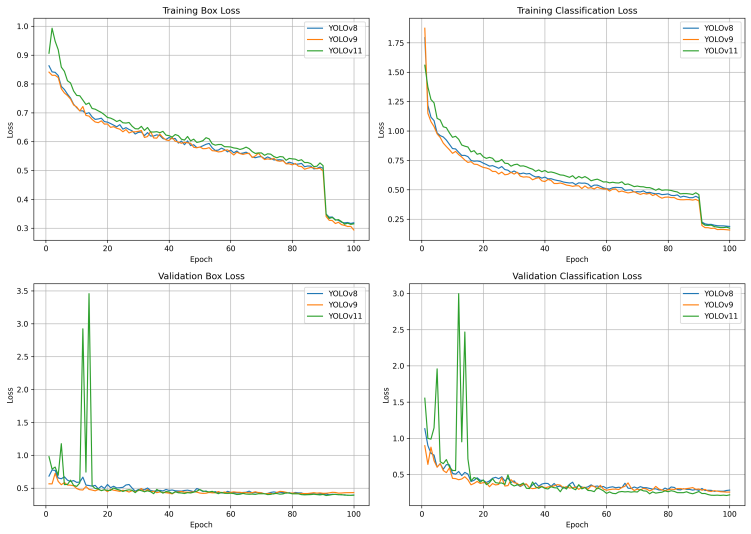
\includegraphics[width=0.9\textwidth]{images/13d4457988945f664ef12271f40e30a3-image.png}}
\caption{Training and validation loss curves for YOLOv8, YOLOv9, and YOLOv11 over 100 epochs.}
\label{fig_loss}
\end{figure}

\subsection{Class-wise Performance Analysis}
All classes achieved uniformly high recall values. Money Plant Bacterial Wilt, Money Plant Healthy, and Money Plant Manganese Toxicity each attained perfect recall (1.000) with high precision and mAP@0.5. Snake Plant Anthracnose demonstrated the lowest precision due to false positives, indicating challenges in distinguishing subtle healthy-leaf variations from actual lesions.

\begin{figure}[H]
\centerline{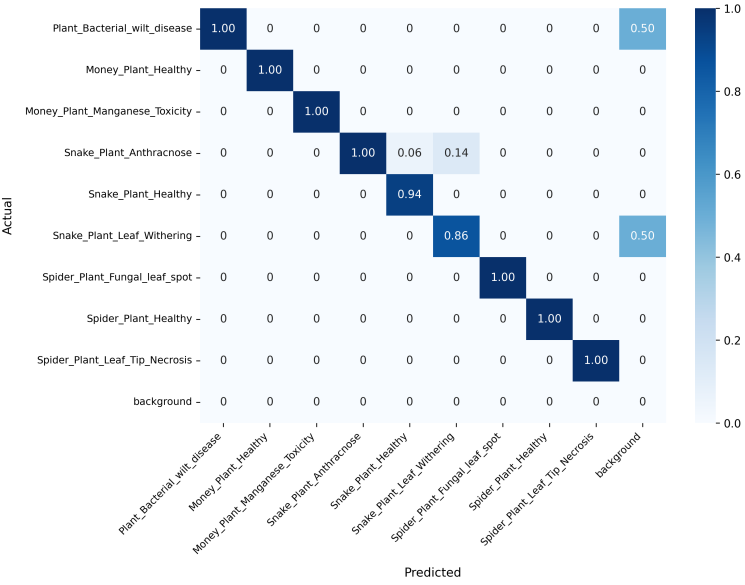
\includegraphics[width=0.7\textwidth]{images/2170dd52fec00de8e34448212b350544-image.png}}
\caption{Normalized confusion matrix for YOLOv11s on the test set.}
\label{fig_confusion}
\end{figure}

\subsection{Model Interpretability Analysis (XAI)}
Occlusion sensitivity systematically masks different regions of the leaf image to observe their effect on model predictions. The resulting heatmaps highlight distributed regions across the leaf surface, demonstrating that YOLOv11 considers global leaf features. RISE generates pixel-level contribution maps, revealing the importance of individual pixels. Higher importance values (red/orange) are concentrated on the leaf tissue areas, indicating that the model focuses on relevant botanical features while suppressing background noise.

\begin{figure}[H]
\centerline{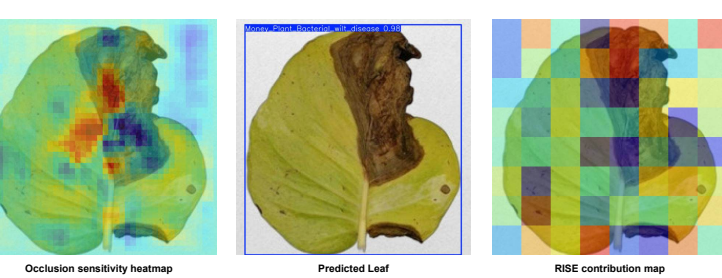
\includegraphics[width=0.8\textwidth]{images/4266e009fcfd001dadcc12d748048091-image.png}}
\caption{Occlusion sensitivity heatmap and RISE contribution map for YOLOv11 on a representative leaf image.}
\label{fig_xai}
\end{figure}

\section{Conclusion}
This work presented a comprehensive framework for detecting and classifying indoor plant leaf diseases using modern YOLO object detection models, fully integrated into a modern software stack. A carefully curated dataset was collected, annotated, and systematically augmented. Comparative evaluation demonstrated that YOLOv11s consistently achieved superior results, attaining 97.4\% mAP@50 and 93.7\% precision. 

By combining this highly accurate model with a Progressive Web App (PWA) architecture built on Next.js and FastAPI, we successfully bridged the gap between academic research and practical deployment. The integration of native camera access, client-side image compression, and real-time inference benchmarking ensures a seamless user experience. Furthermore, interactive Occlusion and RISE heatmaps provide necessary interpretability, proving that the model attends primarily to leaf tissue areas and suppresses background interference. Ultimately, the LeafInsight platform offers a lightweight, accurate, and transparent solution for indoor plant disease monitoring, highly suitable for integration into precision agriculture and mobile plant care systems.

\end{document}
